
%\newcommand{\EntradaBibtex}{DetectorMotos_SistemasInteligentes_UPV_2024}
\renewcommand{\EntradaBibtex}{DetectorMotos_SistemasInteligentes_UPV_2024}

\begin{frame}{\citetitle{\EntradaBibtex}$^*$ (1)}
\begin{block}{Motivación} 
Dada las condiciones de falta de cultura vial en nuestras calles y avenidas, se require de un sistema que permita alertar a un conductor sobre el acercamiento al punto ciego de una motocicleta o el rebase por alguno de los lados del vehiculo. 
\begin{itemize}
\item Se probaron con videos obtenidos de internet
\item Detección de un tipo específico de vehículo (moto)
\item Detectar dicho video en regiones específicas de interes (rebasar por alguno de los lados) 
\end{itemize}
\end{block} 
\footfullcite*{\EntradaBibtex}
\end{frame}


\begin{frame}{\citetitle{\EntradaBibtex} (2)}
%\begin{block}{Pantallas Principales} 

\begin{columns}
% Column 1
\column{.4\linewidth}
\begin{center}
\includegraphics[width=0.85\linewidth]{2024_DetectorMotos/figs/resultados1.png}
\includegraphics[width=0.85\linewidth]{2024_DetectorMotos/figs/resultados2.png}
\end{center}
\column{.6\linewidth}
\begin{center}

	\begin{tabular}{cc}
		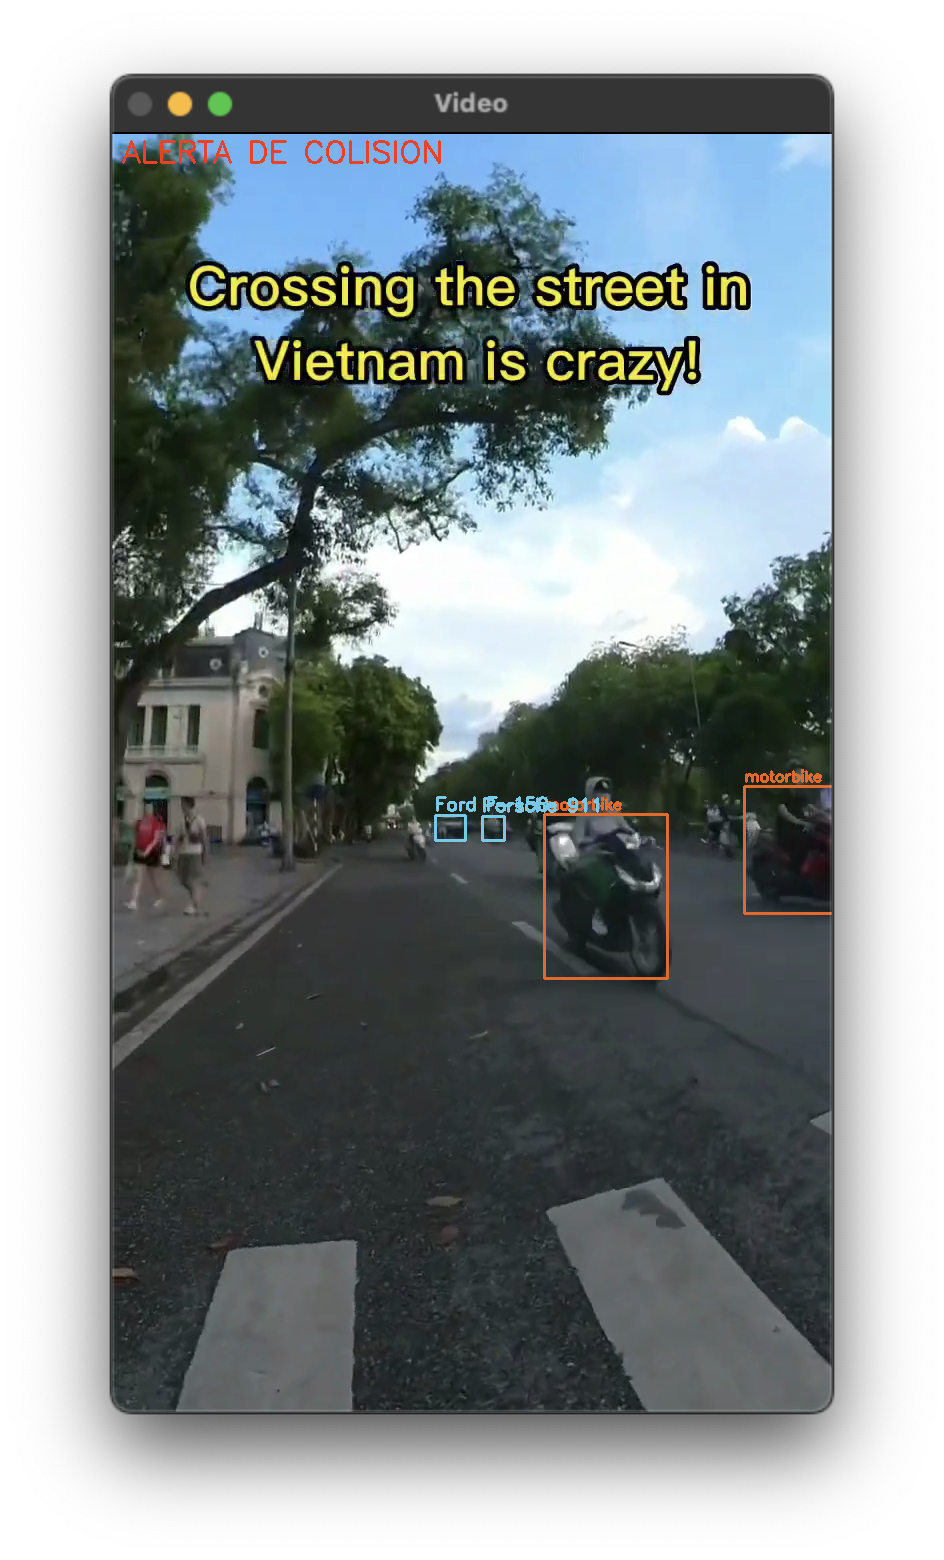
\includegraphics[width=0.49\linewidth]{2024_DetectorMotos/figs/resultados3.png} & 		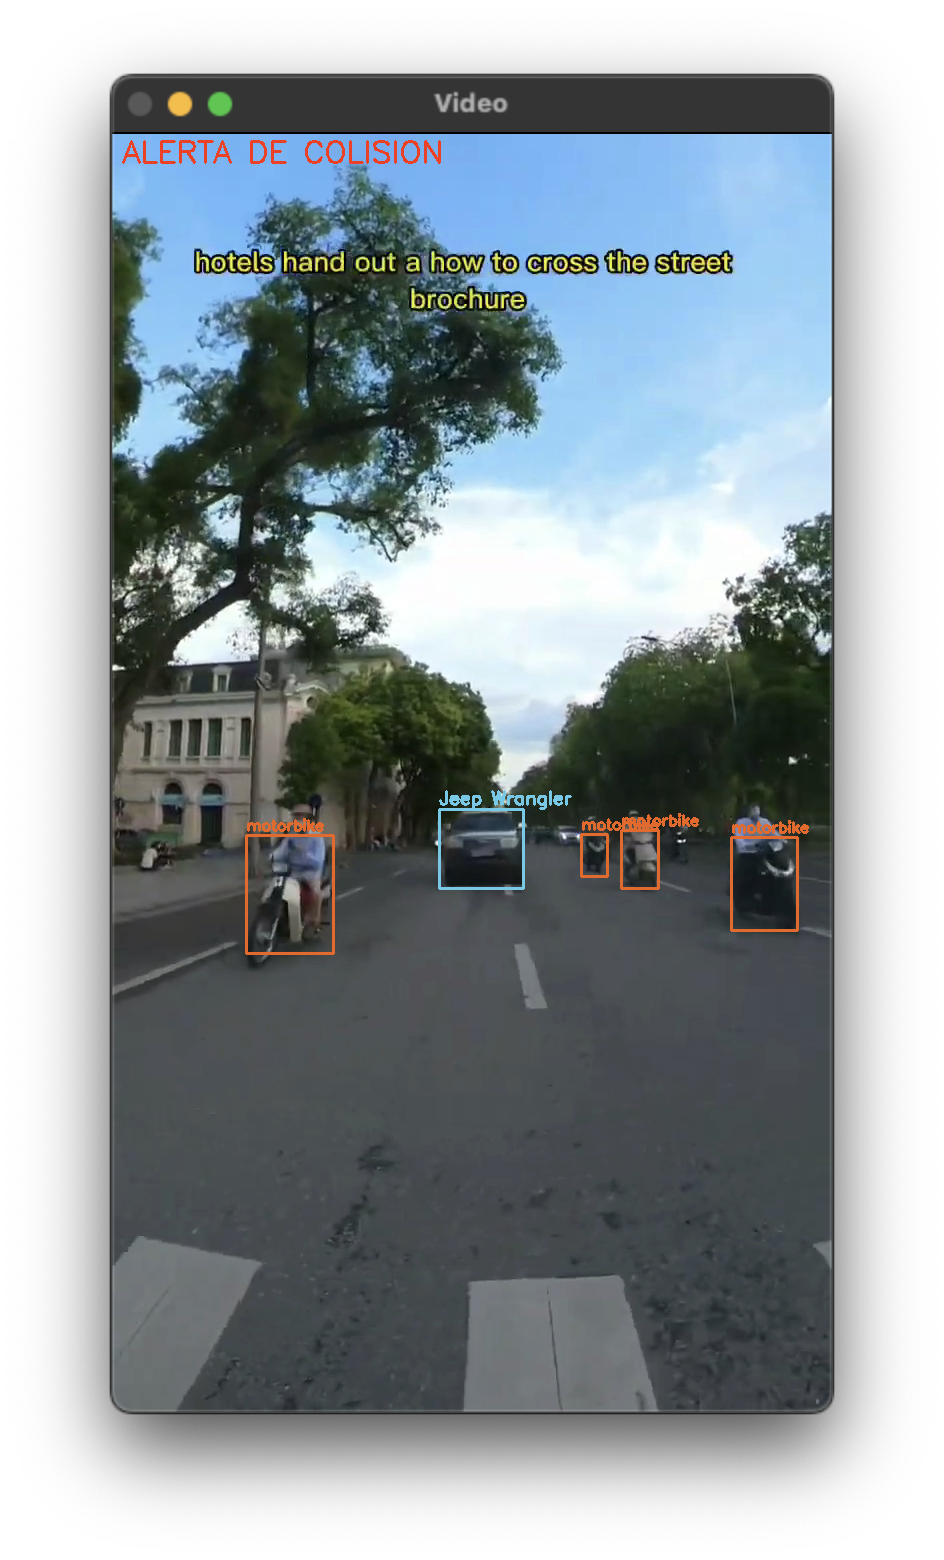
\includegraphics[width=0.49\linewidth]{2024_DetectorMotos/figs/resultados4.png} \\
	\end{tabular}
\end{center}

\end{columns}
\end{frame}


